\index{OpenQuake-engine!Risk}

The seismic risk results are calculated using the \gls{acr:risklib}, 
an open-source suite of tools for seismic risk assessment and
loss estimation. This library is written in the Python programming language
and available in the form of a ``developers'' release at the following location:
\href{https://github.com/gem/oq-engine/tree/master/openquake/risklib}{https://github.com/gem/oq-engine/tree/master/openquake/risklib}.

The risk component of the \glsdesc{acr:oqe} can compute both scenario-based and
probabilistic seismic damage and risk using various approaches. The following
types of analysis are currently supported:

\begin{itemize}

    \item \textit{\textbf{Scenario Damage Assessment}}, for the
	calculation of damage distribution statistics for a portfolio of buildings
	from a single earthquake rupture scenario taking into account aleatory and
	epistemic ground-motion variability.

    \item \textit{\textbf{Scenario Risk Assessment}}, for the calculation of
	individual asset and portfolio loss statistics due to a single earthquake
	rupture scenario taking into account aleatory and epistemic ground-motion
	variability. Correlation in the vulnerability of different assets of the
	same typology can also be taken into consideration.

	\item \textit{\textbf{Classical Probabilistic Seismic Damage Analysis}}, for 
	the calculation of damage state probabilities over a specified time period,  
	and probabilistic collapse maps, starting from the hazard curves 
	computed following the classical integration procedure (\cite{cornell1968}, 
	\citet{mcguire1976}) as formulated by \cite{field2003}.

    \item \textit{\textbf{Classical Probabilistic Seismic Risk Analysis}}, for the
	calculation of loss curves and loss maps, starting from the hazard curves 
	computed following the classical integration procedure (\cite{cornell1968}, 
	\citet{mcguire1976}) as formulated by \cite{field2003}.

	\item \textit{\textbf{Stochastic Event Based Probabilistic Seismic Risk Analysis}}, 
	for the calculation of event loss tables starting from stochastic event sets.
	Other results such as loss-exceedance curves, probabilistic loss maps, 
	and average annual losses can be obtained by 
	post-processing the event loss tables.

    \item \textit{\textbf{Retrofit Benefit-Cost Ratio Analysis}}, which is
	useful in estimating the net-present value of the potential benefits of
	performing retrofitting for a portfolio of assets (in terms of decreased
	losses in seismic events), measured relative to the upfront cost of
	retrofitting.

\end{itemize}

Each calculation workflow has a modular structure, so that intermediate
results can be saved and analyzed. Moreover, each calculator can be
extended independently of the others so that additional calculation options
and methodologies can be easily introduced, without affecting the overall
calculation workflow. Each workflow is described in more detail in the
following sections.

\section{Scenario Damage Assessment}
\index{OpenQuake-engine!Risk calculation workflows!Scenario Damage Assessment}
\label{sec:workflow_scenario_damage}
The scenario damage calculator computes damage distribution statistics for all
\glspl{asset} in a given \gls{exposuremodel} for a single specified
\gls{rupture}. Damage distribution statistics include the mean and standard
deviation of damage fractions for different damage states. This calculator
requires the definition of a finite \gls{rupturemodel}, an \gls{exposuremodel}
and a \gls{fragilitymodel}; the main results are the damage distribution
statistics per \gls{asset}, aggregated damage distribution statistics per
taxonomy, aggregated damage distribution statistics for the region, and
collapse maps, which contain the spatial distribution of the number or area of
collapsed buildings throughout the region of interest.

The \gls{rupture} characteristics---i.e. the magnitude, hypocenter and fault
geometry---are modelled as deterministic in the scenario calculators. Multiple
simulations of different possible \glspl{acr:gmf} due to the single
\gls{rupture} are generated, taking into consideration both the inter-event
variability of ground motions, and the intra-event residuals obtained from a
spatial correlation model for ground motion residuals. The use of logic trees
allows for the consideration of uncertainty in the choice of a ground motion
model for the given tectonic region.

As an alternative to computing the \glspl{acr:gmf} with \glsdesc{acr:oqe},
users can also provide their own sets of \glspl{acr:gmf} as input to the
scenario damage calculator.

\textbf{Note}: The damage simulation algorithm for the scenario damage 
calculator has changed starting from \glsdesc{acr:oqe39} to use a full
Monte Carlo simulation of damage states.

For each \gls{acr:gmf}, a damage state is simulated for each building for every
\gls{asset} in the \gls{exposuremodel} using the provided \gls{fragilitymodel},
and finally the mean damage distribution across all realizations is calculated.
The calculator also provides aggregated damage distribution statistics for the
portfolio, such as mean damage fractions for each taxonomy in the 
\gls{exposuremodel}, and the mean damage for the entire region of study.

The required input files required for running a scenario damage calculation
and the resulting output files are depicted in Figure~\ref{fig:io-structure-scenario-damage}.

\begin{figure}[ht]
\centering
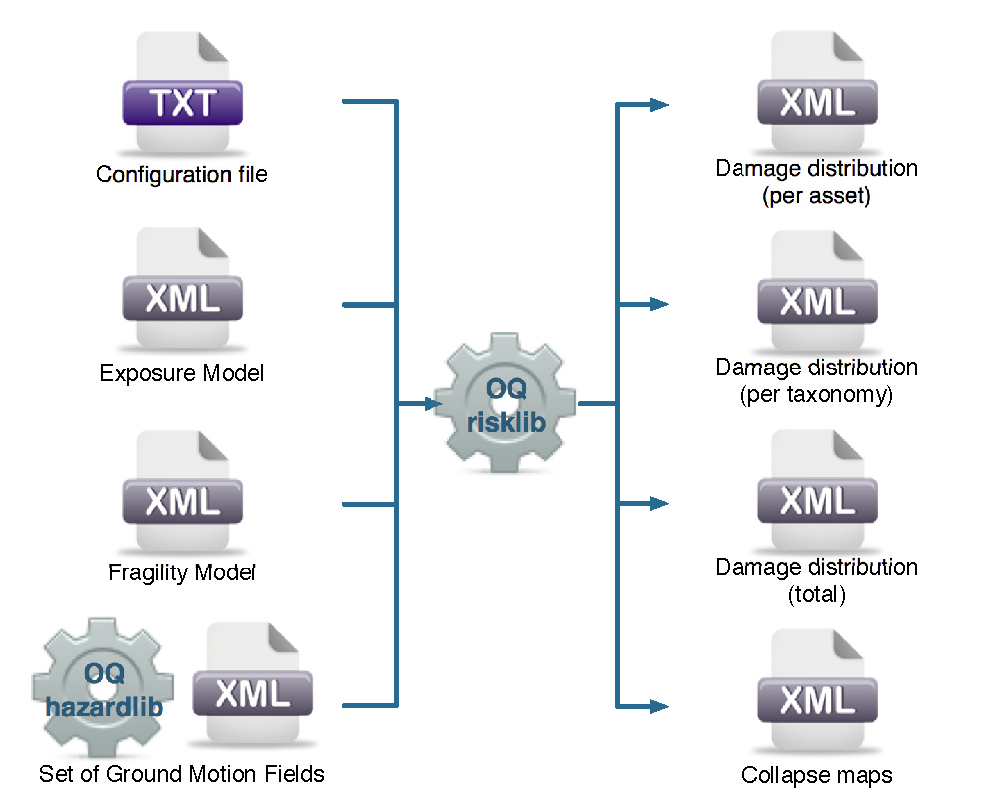
\includegraphics[width=9cm,height=7cm]{figures/risk/io-structure-scenario-damage.pdf}
\caption{Scenario Damage Calculator input/output structure.}
\label{fig:io-structure-scenario-damage}
\end{figure}

\gls{consequencemodel} files can also be
provided as inputs for a scenario damage calculation in addition to
\glspl{fragilitymodel} files, in order to estimate consequences based on the
calculated damage distribution. The user may provide one
\gls{consequencemodel} file corresponding to each loss type (amongst
structural, nonstructural, contents, and business interruption) for which a
\gls{fragilitymodel} file is provided. Whereas providing a
\gls{fragilitymodel} file for at least one loss type is mandatory for running
a Scenario Damage calculation, providing corresponding \gls{consequencemodel}
files is optional.


\section{Scenario Risk Assessment}
\index{OpenQuake-engine!Risk calculation workflows!Scenario Risk Assessment}
\label{sec:workflow_scenario_risk}
The scenario risk calculator computes loss statistics for all \glspl{asset} in
a given \gls{exposuremodel} for a single specified \gls{rupture}.
Loss statistics include the mean and standard deviation of ground-up losses
for each loss type considered in the analysis. Loss
statistics can currently be computed for five different loss types using this
calculator: structural losses, nonstructural losses, contents losses, downtime
losses, and occupant fatalities. This calculator requires the definition of a
finite \gls{rupturemodel}, an \gls{exposuremodel} and a
\gls{vulnerabilitymodel} for each loss type considered; the main results are
the loss statistics per \gls{asset} and mean loss maps.

The \gls{rupture} characteristics---i.e. the magnitude, hypocenter and fault
geometry---are modelled as deterministic in the scenario calculators. Multiple
simulations of different possible \glspl{acr:gmf} due to the single
\gls{rupture} are generated, taking into consideration both the inter-event
variability of ground motions, and the intra-event residuals obtained from a
spatial correlation model for ground motion residuals. The use of logic trees
allows for the consideration of uncertainty in the choice of a ground motion
model for the given tectonic region.

As an alternative to computing the \glspl{acr:gmf} with OpenQuake, users can
also provide their own sets of \glspl{acr:gmf} as input to the scenario risk
calculator.

For each \gls{acr:gmf} simulation, a loss ratio is sampled for every asset in
the \gls{exposuremodel} using the provided probabilistic
\gls{vulnerabilitymodel} taking into consideration the correlation model for
vulnerability of different \glspl{asset} of a given taxonomy. Finally loss
statistics, i.e., the mean loss and standard deviation of loss for
ground-up losses across all simulations, are calculated
for each \gls{asset}. Mean loss maps are also generated by this calculator,
describing the mean ground-up losses caused by the
scenario event for the different assets in the \gls{exposuremodel}.

The required input files required for running a scenario risk calculation and
the resulting output files are depicted in Figure~\ref{fig:io-structure-scenario-risk}.

\begin{figure}[ht]
\centering
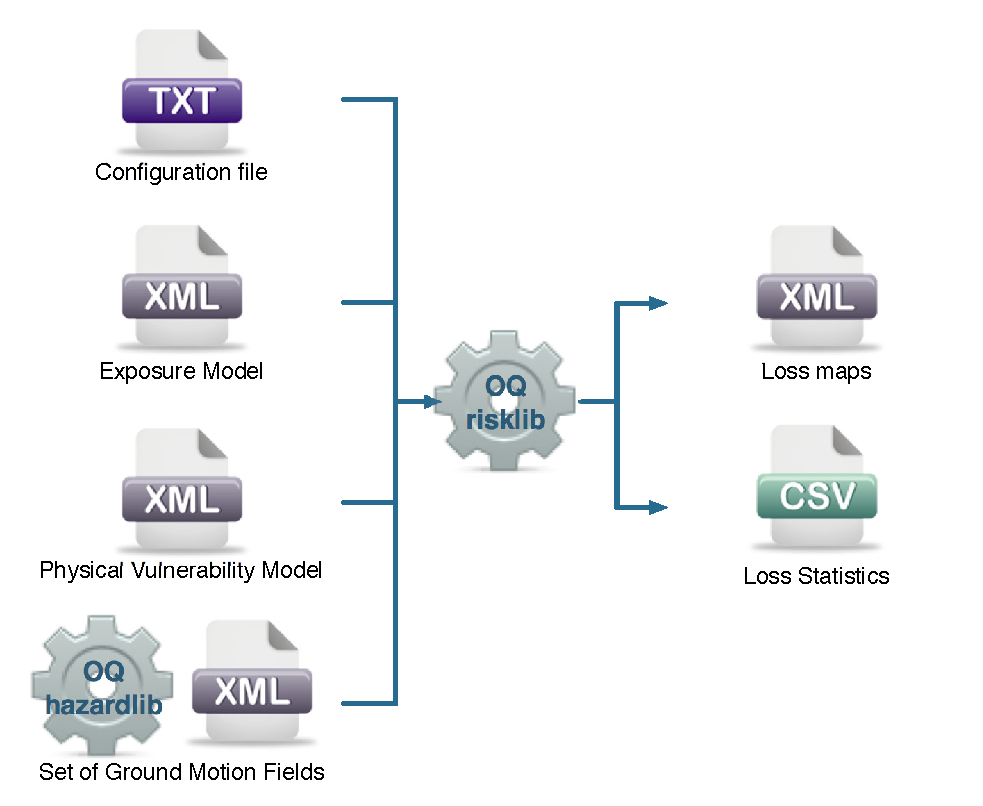
\includegraphics[width=9cm,height=7cm]{figures/risk/io-structure-scenario-risk.pdf}
\caption{Scenario Risk Calculator input/output structure.}
\label{fig:io-structure-scenario-risk}
\end{figure}


\section{Classical Probabilistic Seismic Damage Analysis}
\index{OpenQuake-engine!Risk calculation workflows!Classical Probabilistic Seismic Damage Analysis}
\label{sec:workflow_classical_damage}
The classical PSHA-based damage calculator integrates the fragility functions
for an asset with the seismic hazard curve at the location of the asset, to
give the expected damage distribution for the asset within a specified time
period. The calculator requires the definition of an \gls{exposuremodel}, a
\gls{fragilitymodel} with  \glspl{fragilityfunction} for each taxonomy
represented in the \gls{exposuremodel}, and hazard curves calculated in the
region of interest. The main results of this calculator are the expected
damage distribution for each asset, which describe the probability of the
asset being in different damage states, and collapse maps for the region,
which describe the probability of collapse for different assets in the
portfolio over the specified time period. Damage distribution aggregated by
taxonomy or of the total portfolio (considering all assets in the
\gls{exposuremodel}) can not be extracted using this calculator, as the
spatial correlation of the ground motion residuals is not taken into
consideration.

The hazard curves required for this calculator can be calculated by the
\glsdesc{acr:oqe} for all asset locations in the \gls{exposuremodel} using the
classical PSHA approach \citep{cornell1968, mcguire1976}.

The required input files required for running a classical probabilistic damage
calculation and the resulting output files are depicted in Figure~\ref{fig:io-structure-classical-damage}.

\begin{figure}[ht]
\centering
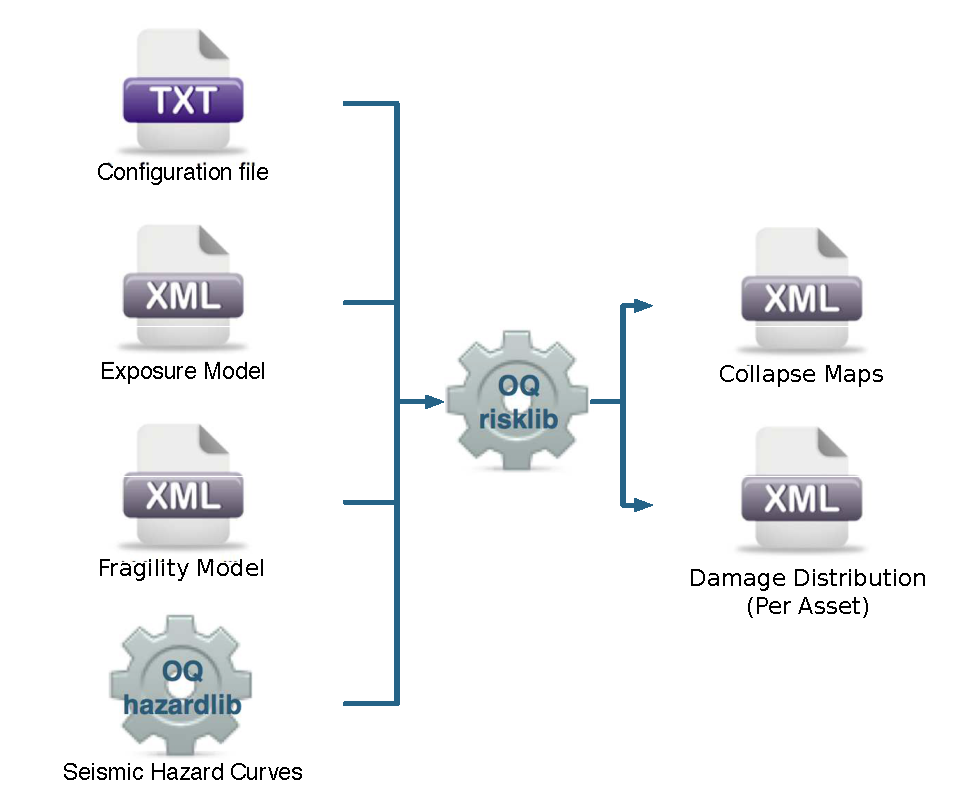
\includegraphics[width=9cm,height=7cm]{figures/risk/io-structure-classical-damage.pdf}
\caption{Classical PSHA-based Damage Calculator input/output structure.}
\label{fig:io-structure-classical-damage}
\end{figure}

\section{Classical Probabilistic Seismic Risk Analysis}
\index{OpenQuake-engine!Risk calculation workflows!Classical Probabilistic Seismic Risk Analysis}
\label{sec:workflow_classical_risk}
The classical PSHA-based risk calculator convolves through numerical
integration, the probabilistic vulnerability functions for an \gls{asset} with
the seismic hazard curve at the location of the asset, to give the loss
distribution for the asset within a specified time period. The calculator
requires the definition of an \gls{exposuremodel}, a \gls{vulnerabilitymodel} for
each loss type of interest with \glspl{vulnerabilityfunction} for each taxonomy
represented in the \gls{exposuremodel}, and hazard curves calculated in the
region of interest. Loss curves and loss maps can currently be calculated for
five different loss types using this calculator: structural losses,
nonstructural losses, contents losses, downtime losses, and occupant
fatalities. The main results of this calculator are loss exceedance curves for
each asset, which describe the probability of exceedance of different loss
levels over the specified time period, and loss maps for the region, which
describe the loss values that have a given probability of exceedance over the
specified time

Unlike the probabilistic event-based risk calculator, an aggregate loss curve
(considering all assets in the \gls{exposuremodel}) can not be extracted using
this calculator, as the correlation of the ground motion residuals and
vulnerability uncertainty is not taken into consideration in this calculator.

The hazard curves required for this calculator can be calculated by the
\glsdesc{acr:oqe} for all asset locations in the \gls{exposuremodel} using the
classical PSHA approach \citep{cornell1968, mcguire1976}. The use of logic-
trees allows for the consideration of model uncertainty in the choice of a
ground motion prediction equation for the different tectonic region types in
the region. Unlike what was described in the previous calculator, a total loss
curve (considering all assets in the \gls{exposuremodel}) can not be extracted
using this calculator, as the correlation of the ground motion residuals and
vulnerability uncertainty is not taken into consideration.

The required input files required for running a classical probabilistic risk
calculation and the resulting output files are depicted in
Figure~\ref{fig:io-structure-classical-risk}.

\begin{figure}[ht]
\centering
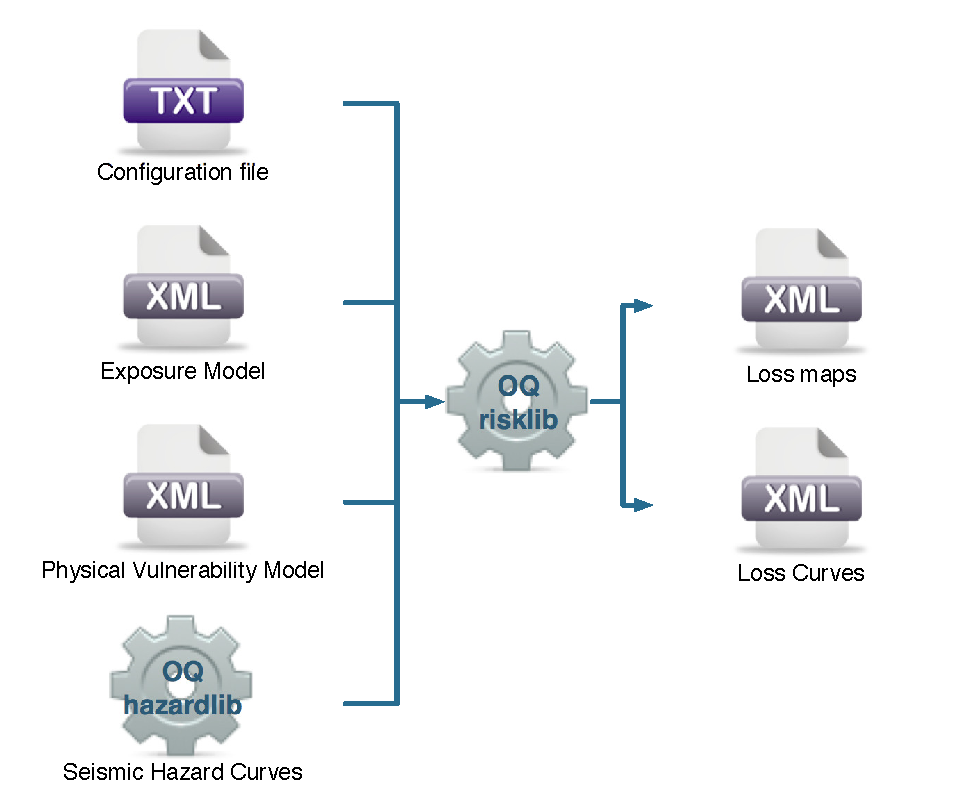
\includegraphics[width=9cm,height=7cm]{figures/risk/io-structure-classical-risk.pdf}
\caption{Classical PSHA-based Risk Calculator input/output structure.}
\label{fig:io-structure-classical-risk}
\end{figure}

\section{Stochastic Event Based Probabilistic Seismic Risk Analysis}
\index{OpenQuake-engine!Risk calculation workflows!Event-Based Probabilistic Seismic Risk Analysis}
\label{sec:workflow_event_based_risk}
This calculator employs an event-based Monte Carlo simulation approach to
probabilistic risk assessment in order to estimate the loss distribution for
individual \glspl{asset} and aggregated loss distribution for a spatially
distributed portfolio of \glspl{asset} within a specified time period. The
calculator requires the definition of an \gls{exposuremodel}, a
\gls{vulnerabilitymodel} for each loss type of interest with
\glspl{vulnerabilityfunction} for each taxonomy represented in the
\gls{exposuremodel}, and a \glsdesc{acr:ses} (also known as a
\textit{synthetic catalog}) representative of the seismicity of the region
over the specified time period. Loss curves and loss maps can currently be
calculated for five different loss types using this calculator: structural
losses, nonstructural losses, contents losses, downtime losses, and occupant
fatalities.

As an alternative to computing the \glspl{acr:gmf} with \glsdesc{acr:oqe},
users can also provide their own sets of \glspl{acr:gmf} as input to the
event-based risk calculator, starting from \gls{acr:oqe28}.

The main results of this calculator are loss
exceedance curves for each \gls{asset}, which describe the probability of
exceedance of different loss levels over the specified time period, and loss
maps for the region, which describe the loss values that have a given
probability of exceedance over the specified time period. Aggregate loss
exceedance curves can also be produced using this calculator; these
describe the probability of exceedance of different loss levels for all
\glspl{asset} in the portfolio. Finally, event loss tables can be produced
using this calculator; these tables describe the total loss across the
portfolio for each seismic event in the \gls{acr:ses}.

This calculator relies on the probabilistic event-based hazard calculator,
which simulates the seismicity of the chosen time period $T$ by producing a
\gls{acr:ses}. For each \gls{rupture} generated by a \gls{seismicsource}, the
number of occurrences in the given time span $T$ is simulated by sampling the
corresponding probability distribution as given by $P_{rup}(k | T)$. A
\gls{acr:ses} is therefore a \textit{sample} of the full population of
\glspl{rupture} as defined by a \glsdesc{acr:ssm}. Each \gls{rupture} is
present zero, one or more times, depending on its probability. Symbolically,
we can define a \gls{acr:ses} as:
\begin{align}
SES(T) = \left\{k \times rup,\;k\sim P_{rup}(k | T)\;\;\forall\;rup\;in\;Src\;\forall\;Src\;in\;SSM\right\}
\end{align}
where $k$, the number of occurrences, is a random sample of $P_{rup}(k | T)$,
and $k \times rup$ means that \gls{rupture} $rup$ is repeated $k$ times in the
\gls{acr:ses}.

For each \gls{rupture} or event in the \glspl{acr:ses}, a spatially correlated
\gls{acr:gmf} realisation is generated, taking into consideration both the
inter-event variability of ground motions, and the intra-event residuals
obtained from a spatial correlation model for ground motion residuals. The use
of logic trees allows for the consideration of uncertainty in the choice of a
\glsdesc{acr:ssm}, and in the choice of \glspl{groundmotionmodel} for the
different tectonic regions.

For each \gls{acr:gmf} realization, a loss ratio is sampled for every
\gls{asset} in the \gls{exposuremodel} using the provided probabilistic
\gls{vulnerabilitymodel}, taking into consideration the correlation model for
vulnerability of different \glspl{asset} of a given taxonomy. Finally loss
exceedance curves are computed for ground-up losses.

The required input files required for running a probabilistic stochastic
event-based risk calculation and the resulting output files are depicted in
Figure~\ref{fig:io-structure-event-based-risk}

\begin{figure}[ht]
\centering
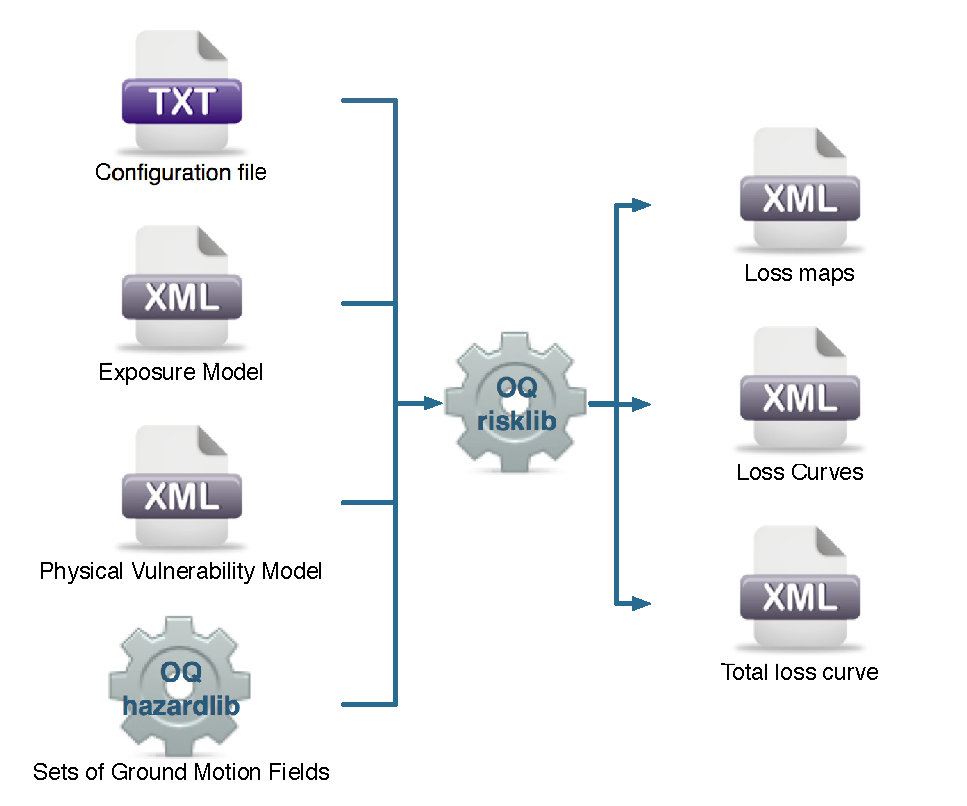
\includegraphics[width=9cm,height=7cm]{figures/risk/io-structure-event-based-risk.pdf}
\caption{Probabilistic Event-based Risk Calculator input/output structure.}
\label{fig:io-structure-event-based-risk}
\end{figure}


\section{Retrofit Benefit-Cost Ratio Analysis}
\index{OpenQuake-engine!Risk calculation workflows!Retrofit Benefit-Cost Ratio Analysis}
\label{sec:workflow_benefit_cost}
This calculator represents a decision-support tool for deciding whether the
employment of retrofitting measures to a collection of existing buildings is
advantageous from an economical point of view. For this assessment, the
expected losses considering the original and retrofitted configuration of the
buildings are estimated, and the economic benefit due to the better seismic
design is divided by the retrofitting cost, leading to the benefit/cost ratio.
These loss curves are computed using the previously described Classical PSHA-
based Risk calculator. The output of this calculator is a benefit/cost ratio
for each asset, in which a ratio above one indicates that employing a
retrofitting intervention is economically viable.

In Figure~\ref{fig:io-structure-benefit-cost}, the input/output structure for
this calculator is depicted.

\begin{figure}[ht]
\centering
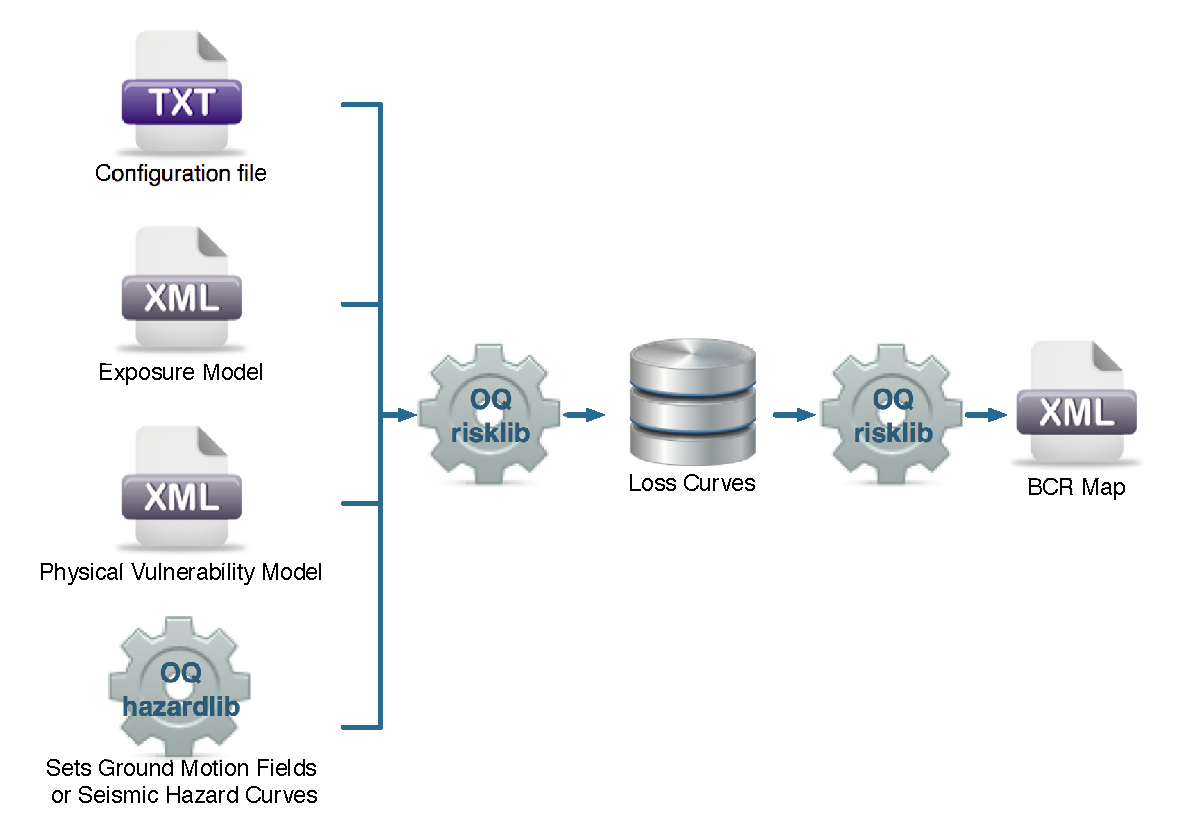
\includegraphics[width=10.5cm,height=7cm]{figures/risk/io-structure-benefit-cost.pdf}
\caption{Retrofitting Benefit/Cost Ratio Calculator input/output structure.}
\label{fig:io-structure-benefit-cost}
\end{figure}

For further information regarding the theoretical background of the
methodologies used for each calculator, users are referred to the OpenQuake-
engine Book (Risk).

\cleardoublepage
